\part{Planejamento}

\chapter[Planejamento]{Planejamento}

\section{Descri\c{c}\~ao do problema}

\begin{figure}[H]
	\centering
	\label{FISHBONE}
		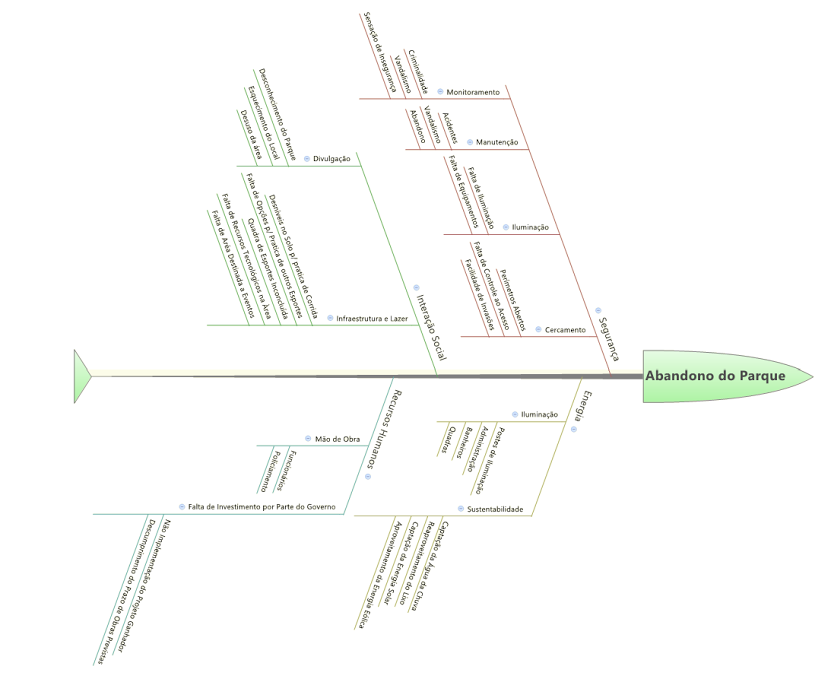
\includegraphics[keepaspectratio=true,scale=0.6]{planejamento/FISHBONE_complete.png}
	\caption{Fishbone do projeto.}
\end{figure}

Os problemas apresentados s\~ao descridos a seguir:

\subsection{Problemas encontrados}

\begin{itemize}
	\item Ilumina\c{c}\~ao: a ilumina\c{c}\~ao \'e um dos grandes problemas do parque. Sem uma ilumina\c{c}\~ao adequada a sensa\c{c}\~ao de seguran\c{c}a \'e m\'inima, dando condi\c{c}\~oes propicias ao crime e consequentemente diminuindo o n\'umero de frequentadores do parque.
	\item Falta de Monitoramento do Parque: o monitoramento do parque \'e quase nulo, muitos lugares estão sendo usados para pr\'aticas de crimes, passando a sensa\c{c}\~ao de abandono do parque com consequ\^encias similares a da falta de ilumina\c{c}\~ao, um bom monitoramento resolveria os problemas do parque, como tamb\'em o da popula\c{c}\~ao das imedia\c{c}\~oes da \'area patrulhada.
	\item Danos na cerca do parque: o cercamento do parque est\'a em condi\c{c}\~oes medianas de conserva\c{c}\~ao, mas possui buracos e em algumas \'areas ele \'e ausente propiciando invas\~oes do terreno, crimes, esconderijos para criminosos e degrada\c{c}\~ao ambiental.
	\item Falta de manuten\c{c}\~ao da infraestrutura: a manuten\c{c}\~ao do parque \'e prec\'aria, com brinquedos quebrados, cal\c{c}adas rachadas al\'em de problemas com a ilumina\c{c}\~ao, isso causa acidentes, evita a pr\'atica de esportes e prejudica o lazer. Solucionando este problema o parque ficaria em boas condi\c{c}\~oes para e uso, evitando reformula\c{c}\~oes do projeto, conservando assim o dinheiro e protegendo a fauna e flora local.
	\item Fonte n\~ao sustent\'avel de energia: n\~ao existe uma fonte sustent\'avel de fornecimento de energia para o parque.
	\item Lixo produzido nos banheiros por usu\'arios e pela administra\c{c}\~ao: o lixo produzido deve ter uma devida destina\c{c}\~ao para n\~ao danificar o local. Este fator \'e extremamente importante, uma vez que o parque \'e considerado reserva ambiental.
	\item A falta de atratividade do parque: a falta de atratividade do parque devido \`a falta de op\c{c}\~ao de recrea\c{c}\~ao, falta de intera\c{c}\~ao entre as pessoas, al\'em de todos os problemas estruturais b\'asicos.
\end{itemize}

\subsection{Quem s\~ao os afetados pelos problemas encontrados}
	
	Os problemas listados podem afetar diretamente ou indiretamente v\'arios p\'ublicos, dentre eles est\~ao a comunidade vizinha ao parque, as crian\c{c}as e jovens que estudam em escolas pr\'oximas. Pessoas que procuram um local para praticar esportes ao ar livre e ter op\c{c}\~oes de lazer e intera\c{c}\~ao social.
	Outro grupo que possivelmente frequenta o parque s\~ao os moradores de rua e habitantes de moradias n\~ao regulamentadas. Sendo assim, policiais, ONG's e agentes governamentais necessitar\~ao estarem presentes.
	Al\'em de toda a comunidade ao redor do parque, que n\~ao necessariamente seja composta apenas por moradores. Incluindo comerciantes, universit\'arios, funcion\'arios do setor p\'ublico em geral que busquem um local de lazer para a os intervalos de trabalho e o fim do expediente.
	Contudo, o local tamb\'em \'e apropriado para receber eventos a n\'ivel distrital devido a sua representatividade e ao espa\c{c}o dispon\'ivel. Afirmando sua caracter\'istica sustent\'avel e ecol\'ogica, o parque buscar\'a repercutir e atrair cada vez mais pessoas.
	
\subsection{Impactos}

Todo problema gera impactos e \'e necess\'ario identificar cada um deles para poder priorizar solu\c{c}\~oes para as causas mais graves. Em seguida s\~ao apresentados impactos observados com o abandono do Parque Urbano do Gama e seus problemas decorrentes:

\begin{itemize}
	\item N\~ao aproveitamento do potencial de atividades que o parque pode oferecer;
	\item A popula\c{c}\~ao n\~ao possui responsabilidade em cuidar, cobrar as autoridades locais;
	\item Ambiental: na forma de polui\c{c}\~ao visual, degrada\c{c}\~ao ambiental, solo, len\c{c}ol fre\'atico;
	\item Presen\c{c}a de usu\'arios de entorpecentes;
	\item Inseguran\c{c}a;
	\item Crimes nas redondezas;
	\item Degrada\c{c}\~ao do patrim\^onio p\'ublico;
	\item Degrada\c{c}\~ao ambiental;
	\item Acidentes;
\end{itemize}

\subsection{5W2H}

A primeira atividade realizada pelo grupo foi responder o 5W2H para ter no\c{c}\~oes iniciais das motiva\c{c}\~oes, causas entre outras informa\c{c}\~oes relacionadas ao projeto. A seguir est\~ao as respostas estabelecidas pelo grupo.

\begin{itemize}
	\item What? (O que ser\'a entregue?): ser\'a entregue um projeto de revitaliza\c{c}\~ao de um parque urbano, em que ser\'a utilizada a tecnologia como principal ferramenta.
	\item Why? (Por qu\^e est\'a sendo feito?): Est\'a sendo realizado devido a atual inutiliza\c{c}\~ao de um espa\c{c}o p\'ublico que possui grande potencial de servir a comunidade vizinha, com o prop\'osito de uma maior comodidade e incentivo ao acesso a partir das aplica\c{c}\~oes tecnol\'ogicas, o que seria um diferencial em vista de outros parques.
	\item Where? (Onde ser\'a feito/ entregue/ utilizado?): Ser\'a feito no parque vivencial urbano localizado na cidade do Gama do Distrito Federal. Uma regi\~ao de cerrado, n\~ao preservado, em que h\'a invas\~oes ilegais, pista de aeromodelismo, problemas de seguran\c{c}a e limpeza.
	\item When? (Quando ser\'a feito/ entregue?): O projeto tem dura\c{c}\~ao de tr\^es meses, tendo como data final de entrega dia 22 de junho de 2015.
	\item Who? (Quem o far\'a?): A realiza\c{c}\~ao deste projeto ser\'a pelos alunos de gradua\c{c}\~ao dos cursos de Engenharia conciliada com empresas interessadas, o Governo do Distrito Federal, \textit{stakeholders} em geral, como a popula\c{c}\~ao interessada.
	\item How? (Como ser\'a realizado?): Ser\'a realizado a partir de pesquisas acerca do tema, reuni\~oes, debates de ideias e utiliza\c{c}\~ao de metodologias de gerenciamento de projetos, como o \textit{SCRUM} e ferramentas de comunica\c{c}\~ao, como o \textit{Trello}.
	\item How much? (Quanto custar\'a?): Analisando, primeiramente a hora-homens trabalhadas, pode-se estimular um valor.

Determinando: 
\begin{itemize}
        \item 9 pessoas ganhando 6 mil
	\item 8 pessoas ganhando 9 mil
	\item 8 pessoas ganhando 4 mil
\end{itemize}

semanalmente 8 horas trabalhadas --- um m\^es 32 horas
acrescentando 25\% de risco

Tem-se : R\$ 197500,00 o que corresponde em hora/m\^es a R\$ 246,32.
\end{itemize}

\section{Justificativa}

A principal motiva\c{c}\~ao do projeto consiste no abandono do parque pela popula\c{c}\~ao e pelo governo, resultando na falta de aproveitamento do parque, em seu potencial social, ecológico e turístico. Com a devida revitaliza\c{c}\~ao, o parque poderia acrescentar op\c{c}\~oes de intera\c{c}\~ao social para o Gama, favorecendo os moradores da cidade e a todos que possam frequent\'a-la.
Devido a essa motiva\c{c}\~ao o que se encontra na realidade do parque s\~ao problemas de seguran\c{c}a, limpeza, o que acarreta baixa especula\c{c}\~ao imobili\'aria em torno e invas\~oes. 

\section{Objetivos}

Nesta se\c{c}\~ao est\~ao descritos os objetivos que devem ser atingidos ao final deste projeto.

\subsection{Objetivo Geral}

Buscar solu\c{c}\~oes tecnol\'ogicas para aumentar a atratividade do parque urbano e vivencial do Gama - DF, aumentando a intera\c{c}\~ao social por parte da popula\c{c}\~ao, fornecendo lazer, sustentabilidade, seguran\c{c}a e preservando a natureza do local. 

\subsection{Objetivos Espec\'{\i}ficos}

Integrar os cursos de engenharia: automotiva; aeroespacial; energia; eletr\^onica e software em que situam os alunos a projetar, colocar em pr\'atica conceitos estudados. 
Apresentar um planejamento de como executar a revitaliza\c{c}\~ao tecnol\'ogica. Relacionar os aspectos f\'isicos e burocr\'aticos que se encontram na regi\~ao atualmente, e as obras j\'a iniciadas pela Administra\c{c}\~ao Regional do Gama; com as legisla\c{c}\~oes distritais que limitam no tocante ao meio ambiente, a popula\c{c}\~ao vizinha e os impactos urbanos. 